\section{Validierung}
Damit das Verhalten des gebauten Baluns getestet werden kann, werden die beiden Aufgaben, die Impedanzanpassung und das Erzwingen symmetrischer Ströme, unabhängig voneinander überprüft.
\subsection{Impedanzanpassung}
Um die Impedanzanpassung zu verifizieren, wurde am Ausgang des Baluns eine Last von \SI{200}{\Omega} angeschlossen. Da es sich um einen Guanella-Balun mit einem Übersetzungsverhältnis von 1:4 handelt, muss man am Eingang nun eine Impedanz von \SI{50}{\Omega} sehen. Dies wurde mit zwei Messungen überprüft.

\paragraph{Impedanzmessung}
Mit folgender Messanordnung wurde die Impedanz des Baluns direkt gemessen. Das Messresultat ist in Abbildung \ref{fig:Eingangsimpedanz2} ersichtlich.
\begin{figure}[H]
	\centering
	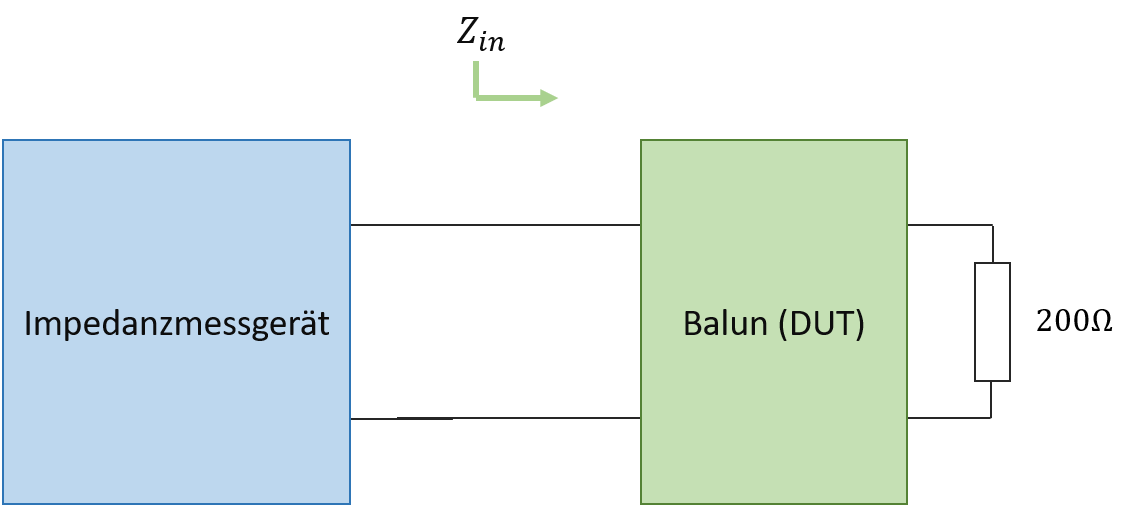
\includegraphics[width=0.6\linewidth]{Messaufbau_Eingangsimpedanz_2.png}
	\caption{Eingangsimpedanz in logarithmischer Darstellung}\label{fig:mess_eingangsimpedanz2}
\end{figure}

\begin{figure}[H]
	\centering
	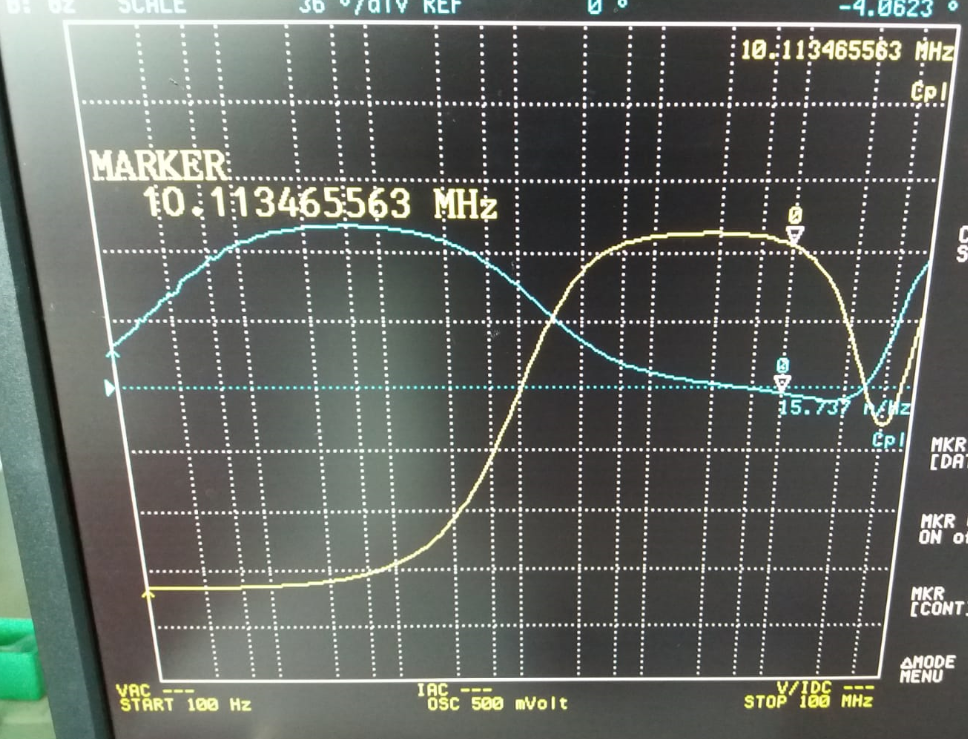
\includegraphics[width=0.6\linewidth]{Eingangsimpedanz2.PNG}
	\caption{Eingangsimpedanz in logarithmischer Darstellung}\label{fig:Eingangsimpedanz2}
\end{figure}
Liegt die gemessene Impedanz in der Nähe von \SI{50}{\Omega} funktioniert die Impedanzanpassung. Wie zu erkennen ist, ist dies im Bereich zwischen \SI{200}{kHz} und \SI{10}{MHz} der Fall. Bei tiefen Frequenzen funktioniert die Impedanzanpassung nicht, weil die Wirkung der einzelnen Wicklungen noch zu schwach ist. Bei höheren Frequenzen beginnt die Wicklungskapazität zu wirken.

\paragraph{Reflexionsmessung}
Auch hier wird überprüft, ob die Eingangsimpedanz \SI{50}{\Omega} beträgt. Dazu wird der Balun in ein \SI{50}{\Omega}-Netzwerk integriert und auf Reflexionen untersucht. Die dafür verwendete Messschaltung ist in Abbildung \ref{fig:mess_eingangsimpedanz} gezeigt.
\begin{figure}[H]
	\centering
	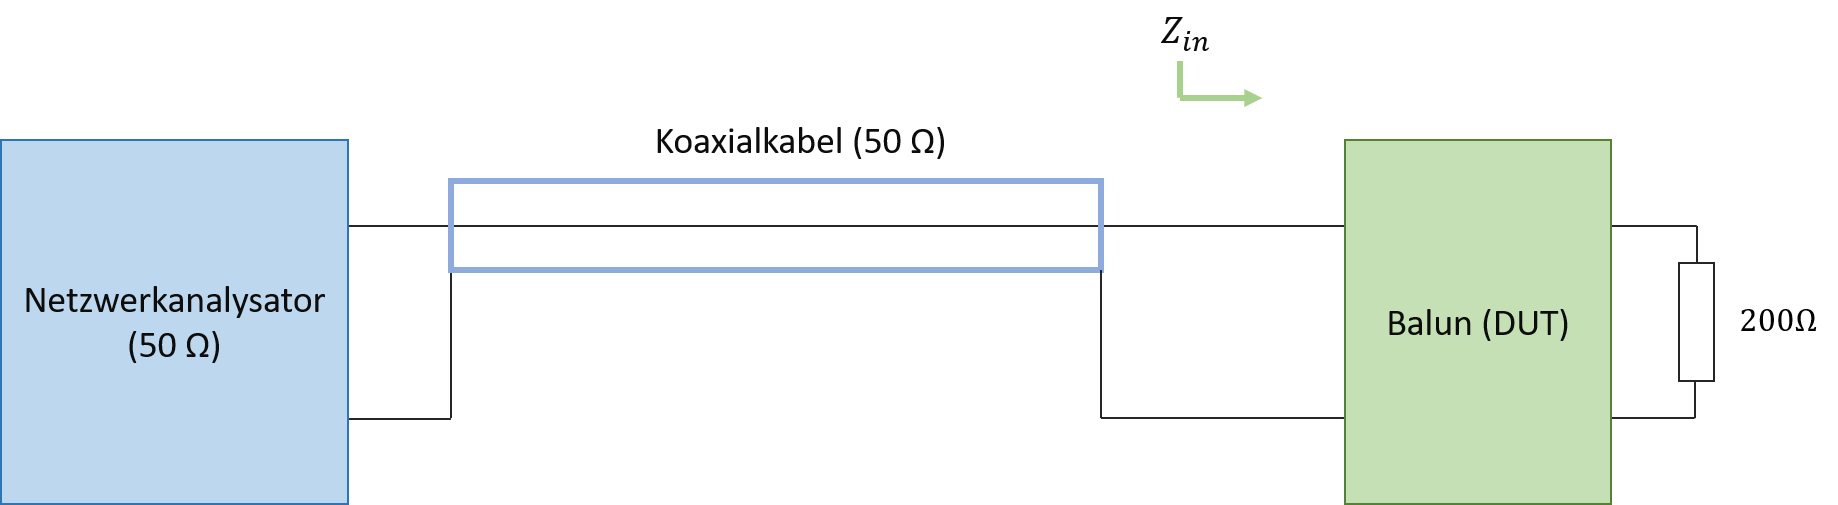
\includegraphics[width=0.7\linewidth]{Messaufbau_Eingangsimpedanz.png}
	\caption{Eingangsimpedanz in logarithmischer Darstellung}\label{fig:mess_eingangsimpedanz}
\end{figure}

\begin{figure}[H]
	\centering
	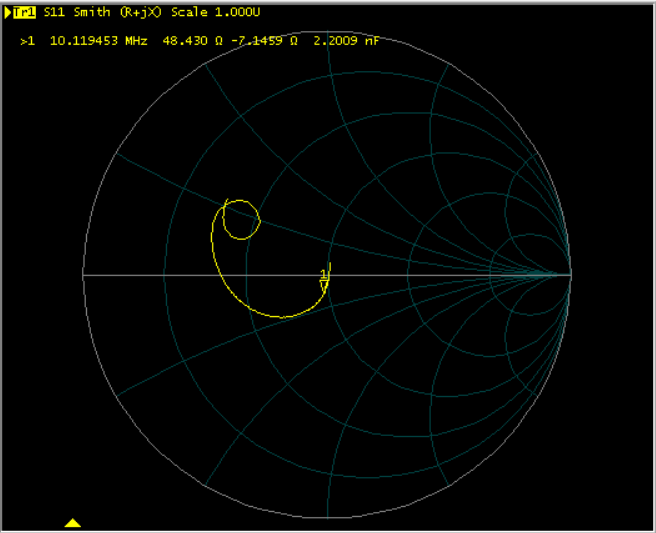
\includegraphics[width=0.7\linewidth]{Eingangsimpedanz.PNG}
	\caption{Eingangsimpedanz dargestellt in der Smith-Chart}\label{fig:Eingangsimpedanz}
\end{figure}

In der Abbildung \ref{fig:Eingangsimpedanz} ist die gemessene Reflexion in der Smith-Chart dargestellt. Wie erwartet, deckt sich das Ergebnis mit der vorherigen Impedanzmessung.
\newpage
\subsection{Symmetrische Ströme}

Um die zweite Aufgabe des Baluns, das Erzwingen symmetrischer Ströme, zu verifizieren, haben wir die im folgenden dargestellte Messung durchgeführt.
\begin{figure}[H]
	\centering
	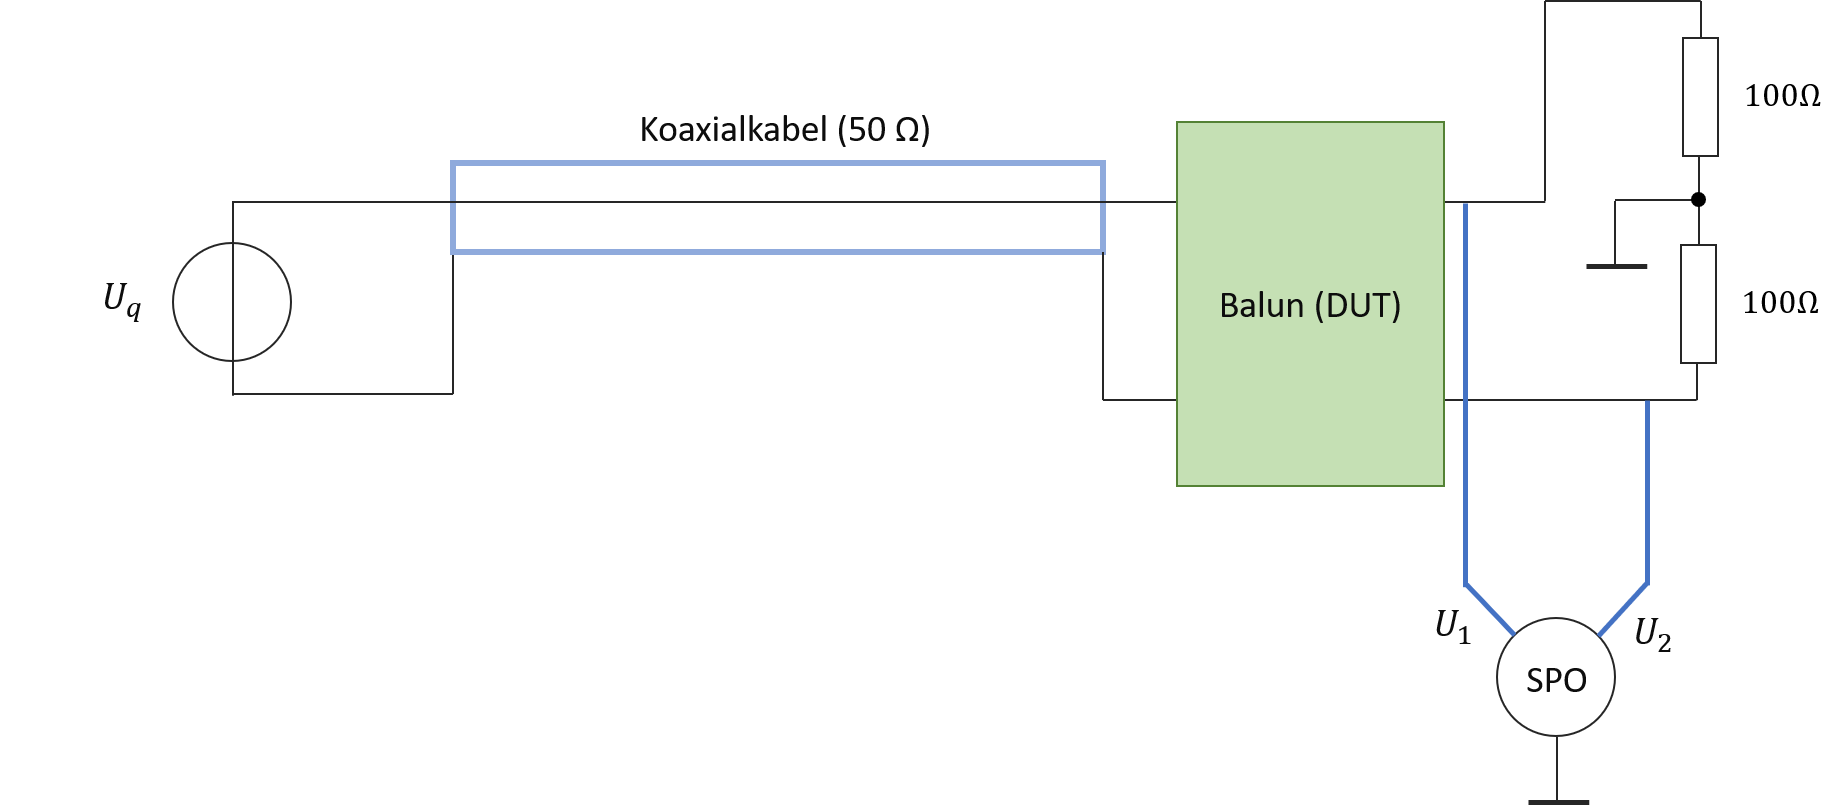
\includegraphics[width=0.8\linewidth]{Messaufbau_Symetrie_1.png}
	\caption{Eingangsimpedanz dargestellt in der Smith-Chart}\label{fig:mess_sym}
\end{figure}
Die beiden Widerstände am Ausgang bilden eine symmetrische Last. Ohne Balun würde die gesamte Spannung über einem der Widerstände abfallen. Bei korrekter Funktion des Baluns liegt an beiden Widerständen die selbe Spannung mit einer Phasenverschiebung von \SI{180}{^\circ} an.\\
In folgender Abbildung ist das Verhältnis der beiden Amplitudenbeträge dargestellt. Man erkennt, dass der Balun zwischen \SI{5}{MHz} und \SI{80}{MHz} symmetrische Stromamplituden erzeugt.

\begin{figure}[H]
	\centering
	\includegraphics[width=0.8\linewidth]{Betrag_Sym.PNG}
	\caption{Eingangsimpedanz dargestellt in der Smith-Chart}\label{fig:Betrag_sym}
\end{figure}
Nun wird überprüft, ob die Phasenverschiebung \SI{180}{^\circ} beträgt. Wie man in Abbildung \ref{fig:Phase_sym} erkennen kann, ist dies praktisch über dem ganzen Messbereich der Fall.
\begin{figure}[H]
	\centering
	\includegraphics[width=0.8\linewidth]{Phase_Sym.PNG}
	\caption{Eingangsimpedanz dargestellt in der Smith-Chart}\label{fig:Phase_sym}
\end{figure}